\documentclass[14pt]{beamer}
\usepackage[utf8]{inputenc}
\usepackage[T1]{fontenc}
\usepackage{lmodern}
\usepackage{amsmath}
\usepackage{amsfonts}
\usepackage{amssymb}
\usepackage{graphicx}
\usetheme{Madrid}
\usecolortheme{beaver}
\usepackage{tabulary}

\newcommand\e{\emph}
\newcommand\tb{\textbf}
\newcommand\un{\underline}
\newcommand\txt{\texttt}

\AtBeginSection[]{
	\begin{frame}
	\vfill
	\centering
	\begin{beamercolorbox}[sep=8pt,center,shadow=true,rounded=true]{title}
		\usebeamerfont{title}\insertsectionhead\par%
	\end{beamercolorbox}
	\vfill
\end{frame}
}

\begin{document}
\author[D. Christenson, J. Lin, and T. Makse] % (optional)
{Dino P. Christenson\inst{1}, Jennifer Lin\inst{2}, and Todd Makse\inst{3}}
\institute[] % (optional)
{
	\inst{1}%
	Faculty of Political Science\\
	Boston University
	\and
	\inst{2}%
	Undergraduate Student\\
	New College of Florida
	\and
	\inst{3}
	Faculty of Political Science\\
	Florida International University
}
\title[Demands for Representation]{Group Interests, Constituency Characteristics and Demands for Representation}
	%\subtitle{}
	%\logo{}
	\date[FPSA 2019]{Florida Political Science Association, March 2019}
	%\subject{}
	\setbeamercovered{transparent}
	\setbeamertemplate{navigation symbols}{}
	\begin{frame}[plain]
	\maketitle
\end{frame}


\begin{frame}
\frametitle{Guiding Questions}
\begin{enumerate}
	\item How does one's social identity influence their demands for representation?
	\item How does knowledge of the district's constituency characteristics influence one's demands for government responsiveness? 
\end{enumerate}
\end{frame}

\begin{frame}
\frametitle{Past Research}
\begin{itemize}
	\item People demand representatives to represent them based on the most salient aspects of their personal identities
	\item Not many are as politically sophisticated to understand how politicians prioritize representation
	\item Citizens may not be as knowledgeable about national politics, but they know what people in their inner circle desire from the national government
	\item Collective v. Dyadic representation - Legislator like me rather than a legislator like my country
\end{itemize}
\end{frame}

\begin{frame}
\footnotesize
\frametitle{Hypotheses}
\begin{enumerate}
	\item \tb{\e{Egocentric Hypothesis:}} As a representative's effort on behalf of groups with which the citizen identifies increases, the citizen's evaluation of the representative will become more positive. 
	\item \tb{\e{Proportionality Hypothesis:}} Citizens will expect that representatives expend effort on behalf of groups in proportion to their role in the constituency.
	\item \tb{\e{Heterogeneity Information Hypothesis:}} The link between representative effort, citizen identity and citizen evaluations will be attenuated by information about the heterogeneity of one’s constituency and strengthened by information about the homogeneity of one’s constituency. 
	\item \tb{\e{Size Information Hypothesis:}} The link between representative effort, citizen identity and citizen evaluations will be attenuated by information that the identity group is a small part of the constituency and strengthened by information that the identity group is a large part of the constituency. 
\end{enumerate}
\end{frame}

\section{Study 1}
\begin{frame}
\frametitle{Experimental Design}
\begin{itemize}
	\item Participants were recruited from Introductory Political Science class and provided ZIP codes - 26 congressional districts represented
	\item Tasks of Representatives
	\item Closeness to group and perceptions of influence
	\item Demands for Effort
	\item District Homogeneity and Effects on Demands 
\end{itemize}
\end{frame}

\begin{frame}
\frametitle{Tasks of Representatives}
\small
\begin{center}
	\e{Thinking about some of the tasks that members of Congress must perform, which of the following tasks would you consider to be somewhat or very challenging, and which would you consider somewhat or very routine?}
\end{center}
\begin{itemize}
	\item Balancing the needs of diverse constituencies - 53\% 
	\item Writing legislation - 27\%
	\item Voting on legislation/Communication with constituents - 11\%
\end{itemize}
\end{frame}

\begin{frame}
\frametitle{Closeness to Groups}
\small
\begin{center}
	\e{Individuals often feel close to certain groups in society, either for personal, social or familial reasons. For each of the following groups, please indicate whether you feel very close to the group, feel somewhat close to the group, or do not feel close to the group.}
\end{center}
\begin{itemize} \itemsep -2pt
	\item College Students
	\item Small business
	\item Military
	\item Elderly
	\item The Poor
	\item Farmers
	\item Unions
\end{itemize}
\end{frame}

\begin{frame}
\frametitle{Distribution of Group Attachment}
\scriptsize
\begin{table}
	\centering
	\caption{Distribution of Group Attachment}
	\begin{tabulary}{\linewidth}{lc c c c}
		\\
		\hline 
		\tb{Group Interest}&\tb{Very Close}&\tb{Somewhat Close}&\tb{Not Close}&\tb{Partisan Gap*}\\
		\hline
		College Students&84\%&12\%&4\%&-0.01\\
		Small Business&26\%&44\%&30\%&0.17\\
		The Military& 23\%&37\%&40\%&0.22\\
		The Elderly&16\%&59\%&25\%&0.14\\
		The Poor&11\%&45\%&43\%&-0.22\\
		Farmers&10\%&30\%&60\%&0.17\\
		Unions&8\%&21\%&71\%&-0.12\\
		\hline
	\end{tabulary}\\
	*Partisan gap indicates the difference between Republicans and Democrats’ propensity to identify with the group. A score of 1.0 would indicate all Republicans very closely identify with the group and all Democrats do not feel close to the group, while a -1.0 would indicate the opposite.
\end{table}
\end{frame}

\begin{frame}
\frametitle{Perception of Influence}
\begin{center}
	\e{Thinking about each of the following groups, how much influence would you think this group might have in your member of Congress' district? Would you say they have a great deal of influence, a moderate amount of influence, a small amount of influence, or virtually no influence?}
\end{center}
\end{frame}

\begin{frame}
\frametitle{Perceived Group Influence in Constituency}
\begin{figure}
	\centering
	{\includegraphics[width=.8\textwidth]{fig1color}}
\end{figure}
\end{frame}

\begin{frame}
\frametitle{Demand for Effort}
\small
\begin{center}
 \e{Please tell us how strongly you agree or disagree with the following statements. Again, with respect to each of the following groups, how would you respond to the statement "I would not consider a member of Congress a good representative unless they exerted major legislative effort on behalf of [Insert groups from Group Attachment Measure]"}
\end{center}
\end{frame}

\begin{frame}
\frametitle{Demands for Representational Effort}
\begin{figure}
	\centering
	{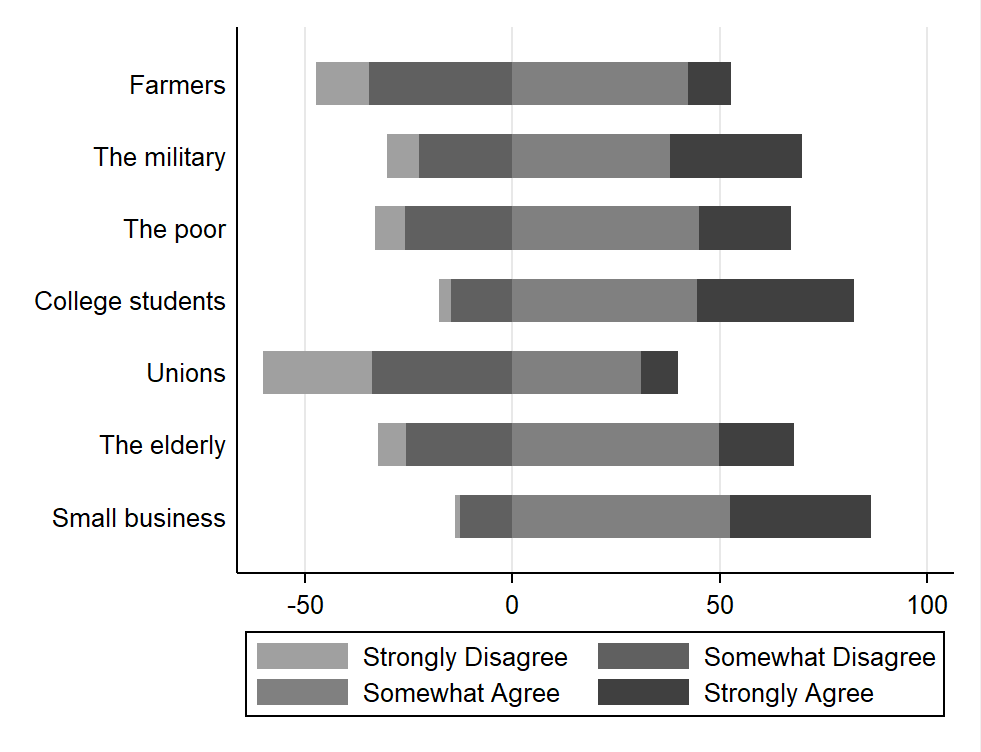
\includegraphics[width=.8\textwidth]{Figure2}}
\end{figure}
\end{frame}

\begin{frame}
\frametitle{Experimental Vignettes}
\begin{itemize}
	\item 2 versions for participant's own district
	\item Homogeneity condition - Emphasis on district homogeneity
	\item Heterogeniety condition - emphasis on diversity in district
	\item Facts were based on data reported by the US Census Bureau and the \e{Almanac of American Politics}
\end{itemize}
\end{frame}

\begin{frame}
\frametitle{Experimental Condition Vignette - Example}
\scriptsize
\begin{table}
	\centering
	\begin{tabulary}{\linewidth}{p{5.5cm}p{5.5cm}}
	\\
	\hline
	\tb{Homogeneity Condition}&\tb{Heterogeneity Condition} \\
	\hline
	Based on the information provided, your member of Congress is Mike Turner, a member of the Republican Party. He has served in Congress since 2003. The Third District of Ohio is a largely urban district which is dominated by the city of Dayton; more than three-quarters of its population resides within Montgomery County. The district is heavily Republican: it has supported Republican presidential candidates in the last three elections, and Turner has not faced a competitive election since being elected to Congress. The district is also racially homogeneous: whites make up more than 80\% of the district’s residents, and this number rises to over 90\% outside of Dayton proper.&Based on the information provided, your member of Congress is Mike Turner, a member of the Republican Party. He has served in Congress since 2003. The Third District of Ohio stretches across large sections of southwestern Ohio, from the city of Dayton to rural counties east of Cincinnati. Although Dayton is the largest city in the district, a majority of its residents live in the Cincinnati media market. The district leans Republican in presidential and Congressional elections, but had a history of electing Democrats to Congress throughout the 1980s and 1990s, and the city of Dayton provides a strong based of Democratic support. The district ranks as one of the most racially diverse in the state of Ohio, with the city of Dayton almost evenly split between black and white residents.\\
	\hline
	\end{tabulary}
\end{table}
\end{frame}

\begin{frame}
\frametitle{Analysis and Results}
\footnotesize
\begin{itemize} \itemsep -2pt
	\item \tb{Analysis:} Ordered logit models and accounted for errors in individual differences
	\item \tb{Model 1:} Personal attachment to group leads to higher demands for representation (23\%) than group preceived group influence (9\%)
	\item \tb{Model 2:} Framing of district homogeneity does not alter demands for representation - If anything, reminders of district composition leads some respondents to think MCs should not cater to some groups
	\item \tb{Model 3:} Closeness to group and preceived group influence are not influenced by information related to the distribution of the district
	\item \tb{Model 4:} Participants are more likely to support representation for groups and parties that they identify, and this is not influenced by the distribution of interests in their district
\end{itemize}
\end{frame}


\section{Study 2}
\begin{frame}
\frametitle{Experimental Design}
\begin{itemize}
	\item 225 Introductory Psychology students
	\item Tasks of Representatives
	\item Vignettes on representative choice
\end{itemize}
\end{frame}

\begin{frame}
\frametitle{Tasks of Representatives}
\small
\begin{center}
	\e{Thinking about some of the tasks that members of Congress must perform, which of the following tasks would you consider to be somewhat or very challenging, and which would you consider somewhat or very routine?}
\end{center}
\begin{itemize}
	\item Balancing the needs of diverse constituencies - 48\% 
	\item Writing legislation - 44\%
	\item Voting on legislation/Communication with constituents - 18\%
\end{itemize}
\end{frame}

\begin{frame}
\frametitle{Vignettes on Representative Choice}
\begin{itemize}
	\item Used common identity as college students to ascertain their feelings of how politicians justify their voting choices on policy that affect college students
	\item Large (20\%) or small (1\%) proportion of district are college students - manipulation of importance
\end{itemize}
\end{frame}

\begin{frame}
\frametitle{Summary of Experimental Scenarios}
\tiny
\begin{table}
	\centering
	\def\arraystretch{1.5}
	\begin{tabulary}{\linewidth}{lCCC}
	\\
	\hline
	&\tb{Scenario 1}&\tb{Scenario 2}&\tb{Scenario 3}\\
	\hline
	Incumbent Decision&Voting for bill that would cut money for hypothetical university&Leading effort to pass financial reform bill that would cut student loan benefits&Accepting seat on Agriculture Committee in lieu of seat on Education Committee\\
	\hline
	Incumbent Defense&Other groups in district will benefit from the bill’s tax cut provisions&Bipartisanship is valuable; getting things done better than demanding the perfect bill&Agriculture is a large sector in the district; opponent pitting groups against each other\\
	\hline
	Constituency Trait Varied&Size of university, 
	\% of residents affiliated with the university&\% of college graduates in the district who have federal student loans&How rural district is; how large agricultural sector in district is\\
	\hline
	Condition 1&Largest university
	20\% of residents&50\% of graduates&75\% rural --
	Third largest agricultural sector in the country
\\
	\hline
	Condition 2&4th largest university
	1\% of residents&10\% of graduates&30\% rural
-- Agriculture is third largest sector in district
\\
	\hline
	\end{tabulary}
\end{table}
\end{frame}

\begin{frame}
\frametitle{Questions}
\begin{enumerate}
	\item Who was more convincing: Incumbent or Challenger?
	\item Based on the decision, are you more or less likely to support the re-election of this MC?
\end{enumerate}
\end{frame}

\begin{frame}
\frametitle{Results and Analyses}
\begin{itemize}
	\item Participants supported incumbents more even if the incumbent did not necessarily go with their interests
	\item Across the scenarios, people were equally likely to support re-election regardless of importance condition
\end{itemize}
\end{frame}

\begin{frame}
\frametitle{Responses to Experiment Vignettes}
\scriptsize
\begin{table}
	\centering
	\begin{tabulary}{\linewidth}{Lccc}
	\\
	\hline
	&\tb{Scenario 1}&\tb{Scenario 2}&\tb{Scenario 3}\\
	&University Funding& Student Loans&Committee Work\\
	\hline
	\e{Incumbent Has Better Argument}&&&\\
	High Importance Condition&61.0\%&37.9\%&67.7\% \\
	Low Importance Condition&62.6\%&49.2\%&69.4\%\\
	Expected Difference (Sign)& ($-$)&($-$)&($+$)\\
	Observed Difference (S.E.)&$-0.2$ (0.06)&$-0.11$ (0.07) \# &$-0.02$ (0.06)\\
	N&225&225&225\\
	&&&\\
	\e{Vote for Incumbent}&&&\\
	High Importance Condition&51.7\%&42.1\%&61.2\%\\
	Low Importance Condition&50.5\%&41.5\%&65.4\%\\
	Expected Difference (Sign)& ($-$)&($-$)&($+$)\\
	Observed Difference&0.01 (0.07)&0.01 (0.07)&$-0,04$ (0.06)\\
	N&225&225&225\\
	\hline
	\end{tabulary}\\
Note: \# p $<$ 0.10; * p $<$ 0.05; ** p $<$ 0.01
\end{table}
\end{frame}

\section{General Discussion}
\begin{frame}
\frametitle{Conclusions}
\begin{center}
	\large
	\tb{Group Identities Guide Demands for Responsiveness} \\
	\smallskip
	\normalsize 
	Voters favor representatives who cater to their most salient social identities
\end{center}
\begin{itemize}
	\small
	\item Study 1: Closeness to group influences perceptions of what warrants representation 
	\item Study 2: District composition does not do much to influence evaluations demands for representation
\end{itemize}
\end{frame}

\begin{frame}
\footnotesize
\frametitle{Hypotheses Revisited}
\begin{enumerate}
	\item \tb{\e{Egocentric Hypothesis:}} As a representative's effort on behalf of groups with which the citizen identifies increases, the citizen's evaluation of the representative will become more positive. -- \tb{Not Really}
	\item \tb{\e{Proportionality Hypothesis:}} Citizens will expect that representatives expend effort on behalf of groups in proportion to their role in the constituency. -- \tb{No}
	\item \tb{\e{Heterogeneity Information Hypothesis:}} The link between representative effort, citizen identity and citizen evaluations will be attenuated by information about the heterogeneity of one’s constituency and strengthened by information about the homogeneity of one’s constituency. -- \tb{No}
	\item \tb{\e{Size Information Hypothesis:}} The link between representative effort, citizen identity and citizen evaluations will be attenuated by information that the identity group is a small part of the constituency and strengthened by information that the identity group is a large part of the constituency. -- \tb{No}
\end{enumerate}
\end{frame}

\begin{frame}
\frametitle{Future Directions}
\begin{itemize}
	\item Observing results via observational methods 
	\begin{itemize}
		\item Campaigns
		\item Legislative Behavior
		\item Outcome of Future Elections
	\end{itemize}
\end{itemize}
\end{frame}

\section{Discussion and Questions}



\end{document}